\documentclass[a4paper,14pt]{extarticle} % the default "article" class is limited to 12pt, but you can go up to 14, 17 or 20 points if you use the "extarticle" class
\usepackage{cmap} % make LaTeX PDF output copy-and-pasteable
\usepackage[T2A]{fontenc}
\usepackage[utf8]{inputenc}
\usepackage[english,ukrainian]{babel}

\usepackage{amssymb, amsfonts, mathtools, amsmath, enumerate}
\usepackage{indentfirst} % set an additional space before a paragraph at the begining of a new section
\usepackage{setspace}
\usepackage{textcomp}

\usepackage{dsfont} % indicator symbol
\usepackage{leftidx} % this package enables left subscripts and superscripts in math mode

\usepackage{import} % for adding a file by path https://tex.stackexchange.com/questions/246/when-should-i-use-input-vs-include

\usepackage{geometry} 
\geometry{left=1.25cm}
\geometry{right=1.25cm}
\geometry{top=1cm}
\geometry{bottom=2cm}

\setlength{\arrayrulewidth}{0.3mm} % this sets the thickness of the borders of the table
\setlength{\tabcolsep}{12pt} % the space between the text and the left/right border of its containing cell is set to 18pt with this command
\renewcommand{\arraystretch}{1.5} % the height of each row is set to 1.5 relative to its default height

\usepackage[table,xcdraw,dvipsnames]{xcolor}
\usepackage{multirow}
\usepackage{color}
% 1) tutorial about xcolor:  https://www.overleaf.com/learn/latex/Using_colours_in_LaTeX
% 2) huge tutorial about xcolor: https://latex-tutorial.com/color-latex/ 
% 3) RGB calculator: https://www.w3schools.com/colors/colors_rgb.asp

\usepackage{hyperref}
\definecolor{linkcolor}{HTML}{0000FF}
\definecolor{urlcolor}{HTML}{0000FF} 
\hypersetup{pdfstartview=FitH, unicode=true, linkcolor=linkcolor, urlcolor=urlcolor, colorlinks=true}

\usepackage{graphicx}
\usepackage{wrapfig}
\usepackage{float}

\parskip=1mm % space between paragraphs

% enumerating equations according to the section number 
% plus resetting each numeration inside each section
\numberwithin{equation}{section}

% numbering only sections in the table of contents (the "1" nesting level)
% thus numbering equations only according to the section number
\setcounter{secnumdepth}{1}

\usepackage{listingsutf8} % origin: \usepackage{listings}

\lstset{
    frame=single,
    language=Python,
    aboveskip=3mm,
    belowskip=3mm,
    columns=flexible,
    basicstyle=\small\ttfamily,
    numbers=left,
    numberstyle=\tiny\color{gray},
    commentstyle=\color{OliveGreen},
    stringstyle=\color{Mahogany},
    morestring=[b]''',
    showstringspaces=false,
    keywordstyle=\bfseries\color{blue},
    emph={[1]import, as, for, while, return}, emphstyle={[1]\bfseries\color{Mulberry}},
    emph={[2]range}, emphstyle={[2]\bfseries\color{brown}},
    breaklines=true,
    breakatwhitespace=true,
    tabsize=4,
    extendedchars=false, % to use ukrainian text in a code
    inputencoding=utf8 % to use ukrainian text in a code
}

\begin{document}

\import{Title/}{title}

\section*{Теоретична довідка}

Неxай задана послідовність $m$ незалежних випадкових величин $Y_i \sim N(\mu_i, \sigma_i^2)$, кожна з яких має нормальний розподіл. На додачу введемо дискретну випадкову величину $X$ зі значеннями в множині 
$\{ 1,2,\ldots,m \}$, для якої виконується закон розподілу 
$\sum\limits_{i=1}^m p_i = 1$ при значеннях $p_i=P(X=i)$. 

Сумішшю нормальних розподілів $N(\mu_1, \sigma_1^2), \ldots, N(\mu_m, \sigma_m^2)$ зі змішувальними коефіцієнтами 
$(p_i)_{i=\overline{1,m}}$ називають випадкову величину
\[ Z=\sum\limits_{i=0}^{m}Y_i\cdot \mathds{1}(X=i) = \begin{cases}
    Y_1, &\text{при } X=1, \\
    Y_2, &\text{при } X=2, \\
    \ldots \\
    Y_m, &\text{при } X=m \\
\end{cases}\]
із такою щільністю розподілу:
\[ f_Z(t)=\sum\limits_{i=1}^m p_i\ \tfrac{1}{\sqrt{2\pi}\; \sigma_i}\ e^{-\tfrac{(t-\mu_i)^2}{2\sigma_i^2}} \]

Розглянемо EM-алгоримт для задачі оцінки невідомих параметрів деякої суміші нормальних розподілів:
$\theta=(p_1,\ldots, p_m;\ \mu_1,\ldots, \mu_m;\ \sigma_1^2,\ldots, \sigma_m^2)$. Кожна ітерація алгоритму складається із таких кроків:
\begin{enumerate} [(1)]
    \item Ініціалізація: нехай 
    $\theta^{(0)}=(p_1^{(0)},\ldots, p_m^{(0)};\ \mu_1^{(0)},\ldots, \mu_m^{(0)};\ \sigma_1^{2^{(0)}},\ldots, \sigma_m^{2^{(0)}})$ 
    -- деяке початкове наближення шуканих параметрів;
    \item E-крок (expectation): обчислюємо математичне сподівання логарифма функції правдоподібності, використовуючи наближені параметри з попереднього кроку;
    \item M-крок (maximization): вираховуємо значення, яке максимізує щойно знайдене математичне сподівання; 
    \item Крок ітерації: покладаємо покращену оцінку параметрів як точку відліку для наступного витка алгоритму. Припиняємо алгоритм при досягненні певного числа ітерацій або за виконання умов збіжності (які можна досягти у випадку нормального розподілу). 
\end{enumerate}

Наведемо явний вигляд формул переоцінки шуканих $m$ параметрів суміші нормального розподілу для заданої кількості $n$ спостережень $\{Y_k\}_{k\geqslant 1}$:

\[ p_j^{(t+1)}=\frac{1}{n}\sum\limits_{k=1}^n\omega_j(y_k \ |\ \theta^{(t)}), \]

\[ \mu_j^{(t+1)}=\frac{\sum\limits_{k=1}^n y_k \omega_j(y_k \ |\ \theta^{(t)})}
{\sum\limits_{k=1}^n \omega_j(y_k \ |\ \theta^{(t)})}, \]

\[ \sigma_j^{2^{(t+1)}}=\frac{\sum\limits_{k=1}^n (y_k-\mu_j^{(t+1)})^2 \omega_j(y_k \ |\ \theta^{(t)})}
{\sum\limits_{k=1}^n \omega_j(y_k \ |\ \theta^{(t)})}, \]

де величина $\omega_j(y_k \ |\ \theta^{(t)})$ матиме такий вигляд:

\begin{align*}
    &\omega_j(y_k \ |\ \theta^{(t)})=
    \frac{p_j^{(t)} \tfrac{1}{\sqrt{2\pi}\; \sigma_j^{(t)}}\ e^{-\tfrac{(y_k-\mu_j^{(t)})^2}{2\sigma_j^{2^{(t)}}}}}
    {\underbracket{\sum\limits_{i=1}^m p_i^{(t)} \tfrac{1}{\sqrt{2\pi}\; \sigma_j^{(t)}}\ e^{-\tfrac{(y_k-\mu_i^{(t)})^2}
    {2\sigma_i^{2^{(t)}}}}}_{f(y_k | \theta^{(t)})}}
\end{align*}

\section*{Оцінка параметрів суміші двох розподілів}

Нехай згенеровано величини $\{Y_k\}_{k\geqslant 1}$ із суміші такого виду:
\[ \tfrac{2}{3}N(10,1) + \tfrac{1}{3}N(5,1) \]

Зобразимо гістограму та криву набору з $n=500$ елементів:

\begin{figure}[H]
    \center{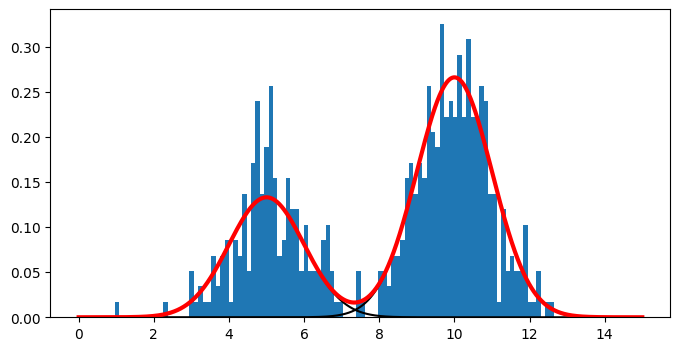
\includegraphics[width=0.9\linewidth]{images/hist2input.png}}
    \caption{Гістограма суміші двох розподілів}
    \label{figure: 2input histogram}
\end{figure}

Програматично таке генерування виконано засобами мови \texttt{Python}: у рядках 2-4 Лістингу \ref{code: generating data} на черговій ітерації до загального масиву величин додається елемент, який згідно заданих імовірностей матиме розподіл або $\tfrac{2}{3}N(10,1)$, або $\tfrac{1}{3}N(5,1)$.

\begin{lstlisting}[firstnumber=1, label = code: generating data, caption = Генерування даних]
    ksi = []
    for i in range(n):
        index = np.argmax(np.random.multinomial(1, p))
        ksi_i = np.random.normal(mu[index], sigma[index])
        ksi.append(ksi_i)
\end{lstlisting}

\vspace{0.4cm}
Наступним етапом застосуємо ЕМ-алгоритм, вважаючи, що параметри суміші $p$ та $\mu=(\mu_1, \mu_2)$ є невідомими, а у нас на руках лише набір з $n$ згенерованих спостережень $\{y_k\}$ та відомі значення дисперсій: $\sigma^2=(\sigma^2_1, \sigma^2_2)=(1, 1)$. Програмна ралізація переоцінки параметів $p$ та $\mu$ зображеня на лістингу нижче:  

\begin{lstlisting}[firstnumber=1, label = code: EM3, caption = Функція EM-алгоритму]
    def EM(Q_previous, y):
    Q = Q_previous

    # overestimation of probabilities
    sum = 0
    for k in range(n):
        f = Q[0]*np.exp(-0.5*pow((y[k]-Q[2]),2)) + (1-Q[0])*np.exp(-0.5*pow((y[k]-Q[1]),2))
        sum += Q[0]*np.exp(-0.5*pow((y[k]-Q[2]),2))/f

    Q[0] = sum/n

    # overestimation of mathematical expectation
    w1, sum_up, sum_down = 0, 0, 0
    for k in range(n):
        f = Q[0]*np.exp(-0.5*pow((y[k]-Q[2]),2)) + (1-Q[0])*np.exp(-0.5*pow((y[k]-Q[1]),2))
        w1 = (1-Q[0])*np.exp(-0.5*pow((y[k]-Q[1]),2))/f
        sum_up += y[k]*w1
        sum_down += w1

    Q[1] = sum_up/sum_down

    w2, sum_up, sum_down = 0, 0, 0
    for k in range(n):
        f = Q[0]*np.exp(-0.5*pow((y[k]-Q[2]),2)) + (1-Q[0])*np.exp(-0.5*pow((y[k]-Q[1]),2))
        w2 = Q[0]*np.exp(-0.5*pow((y[k]-Q[2]),2))/f
        sum_up += y[k]*w2
        sum_down += w2

    Q[2] = sum_up/sum_down

    return Q
\end{lstlisting}

\subsection*{Результати роботи алгоритму}

\subsubsection*{Bід ітерації до ітерації}

Зобразимо результати роботи алгоритму, взявши за початкове наближення, наприклад, такі параметри: 
\[ \theta^{(0)} = (p^{(0)}, \mu_1^{(0)}, \mu_2^{(0)})=(0.8,\ 8,\ 7) \]

\begin{figure}[H]
    \center{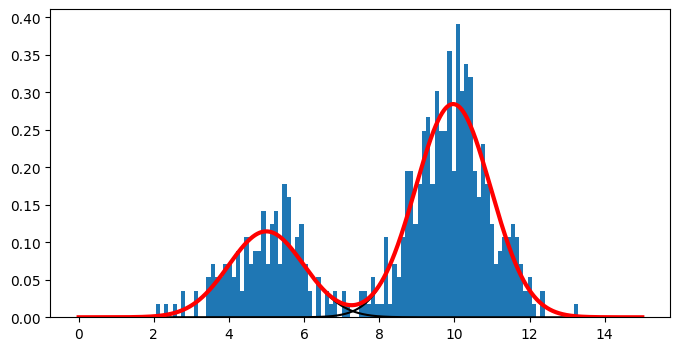
\includegraphics[width=1\linewidth]{images/EM_two_2.png} Ітерація №2: [0.28719535408729163, 9.964985178812421, 4.993402055506498]}
\end{figure}

\begin{figure}[H]
    \center{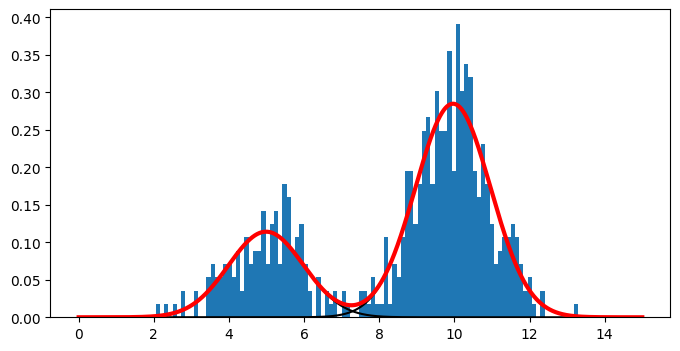
\includegraphics[width=1\linewidth]{images/EM_two_4.png} Ітерація №4: [0.28609300530597354, 9.961857617679273, 4.986958379907583]}
\end{figure}

\begin{figure}[H]
    \center{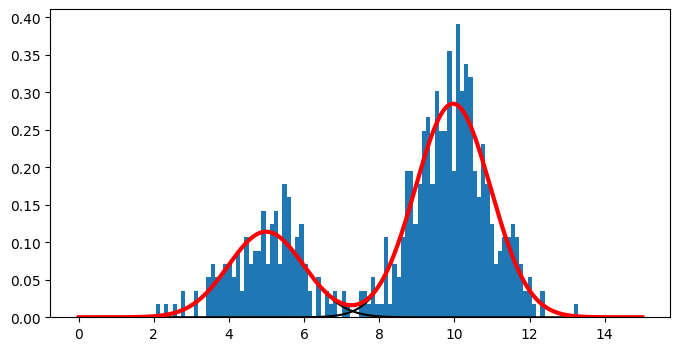
\includegraphics[width=1\linewidth]{images/EM_two_8.png} Ітерація №8: [0.2860821898239672, 9.961825817267654, 4.986907989367006]}
\end{figure}

\begin{figure}[H]
    \center{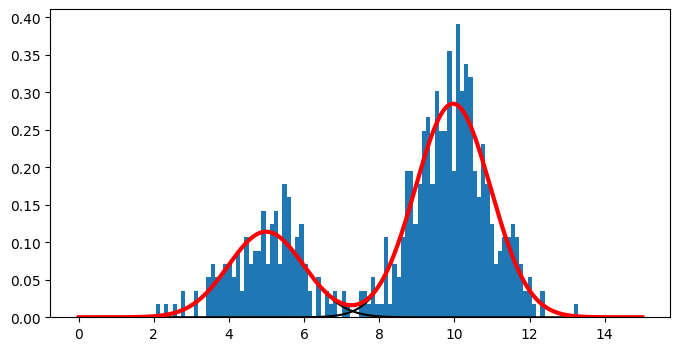
\includegraphics[width=1\linewidth]{images/EM_two_16.png} Ітерація №16: [0.28608218911775435, 9.961825815224344, 4.9869079862629935]}
\end{figure}

\begin{figure}[H]
    \center{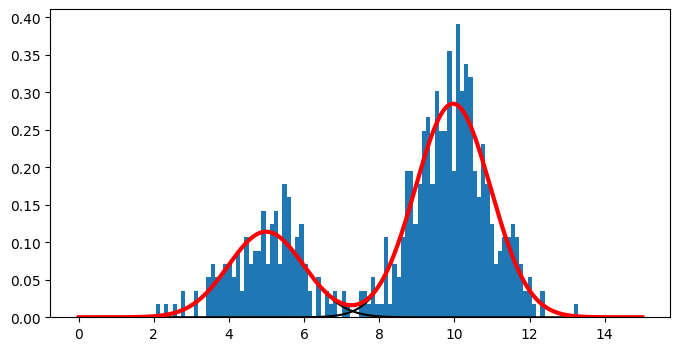
\includegraphics[width=1\linewidth]{images/EM_two_32.png} Ітерація №32: [0.2860821891177544, 9.961825815224342, 4.9869079862629935]}
\end{figure}

\subsubsection*{B залежності від початкового значення}

Зауважимо, що у прикладі вище при $\theta^{(0)} = (p^{(0)}, \mu_1^{(0)}, \mu_2^{(0)})=(0.8,\ 8,\ 7)$ алгоритм демонструє збіжність математичних сподівань із точністю $\varepsilon=0.04$ вже за $k=3$ ітерацій. Прослідкуємо за збіжністю до аналогічної точності в залежності від вибору початкових параметрів суміші: 

\vspace{0.4cm}
\begin{table}[H]
    \begin{center}
        \begin{tabular}{||c|c|c||}
            \hline
            Початкові параметри & Ітерації & Точність \\
            \hline \hline
            $(p^{(0)}=0.8,\ \mu_1^{(0)}=12,\ \mu_2^{(0)}=3)$ & 2 & \multirow{9}{*}{0.04} \\
            $(p^{(0)}=0.8,\ \mu_1^{(0)}=15,\ \mu_2^{(0)}=10)$ & 6 & \\
            $(p^{(0)}=0.8,\ \mu_1^{(0)}=18,\ \mu_2^{(0)}=-2)$ & 3 & \\
            \cline{1-2}
            $(p^{(0)}=0.5,\ \mu_1^{(0)}=12,\ \mu_2^{(0)}=3)$ & 2 & \\
            $(p^{(0)}=0.5,\ \mu_1^{(0)}=15,\ \mu_2^{(0)}=10)$ & 6 & \\
            $(p^{(0)}=0.5,\ \mu_1^{(0)}=18,\ \mu_2^{(0)}=-2)$ & 3 & \\
            \cline{1-2}
            $(p^{(0)}=0.2,\ \mu_1^{(0)}=12,\ \mu_2^{(0)}=3)$ & 2 & \\
            $(p^{(0)}=0.2,\ \mu_1^{(0)}=15,\ \mu_2^{(0)}=10)$ & 6 & \\
            $(p^{(0)}=0.2,\ \mu_1^{(0)}=18,\ \mu_2^{(0)}=-2)$ & 3 & \\
            \hline
        \end{tabular}
        \caption{Порівняння результатів в залежності від початкової точки}
        \label{table: UKR F-test}
    \end{center}
\end{table}

\section*{Оцінка параметрів суміші чотирьох розподілів}

Нехай тепер згенеровано величини $\{Y_k\}_{k\geqslant 1}$ із суміші таких чотирьох нормальних розподілів:
\[ \tfrac{1}{4}N(-20,2^2) + \tfrac{1}{4}N(0,5^2) + \tfrac{1}{4}N(3,4^2) + \tfrac{1}{4}N(10,3^2) \]

Зобразимо гістограму та криву набору з $n=1000$ спостережень (чорним кольором позначено криві окремих складових суміші):

\begin{figure}[H]
    \center{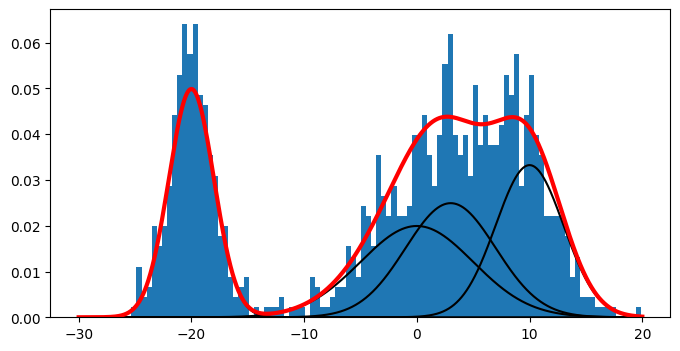
\includegraphics[width=1\linewidth]{images/hist4input.png}}
    \caption{Гістограма суміші чотирьох розподілів}
    \label{figure: 4input histogram}
\end{figure}

Генерування значень відбувається за аналогічною схемою, як це показано на Лістингу \ref{code: generating data}. А от сам алгоритм цього разу реалізовано за загальними формулами, наведеними у пешому розділі теоретичної довідки (тобто для довільної кількості невідомих параметрів):

\begin{lstlisting}[firstnumber=1, label = code: EM, caption = Узагальнена функція ЕМ-алгоритму]
    def EM(Q_previous, y):
        Q = Q_previous

        n = len(y)
        m = len(Q[0])

        # overestimation of probabilities
        for j in range(m):
            f = np.array([0.0 for i in range(n)])
            for k in range(n):
                for i in range(m):    
                    f[k] += Q[0][i]*np.exp(-pow(y[k]-Q[1][i],2)/(2*Q[2][i]**2))/Q[2][i]
                if f[k] == 0.0: f[k] = f.mean()
            sum = 0
            for k in range(n):
                sum += Q[0][j]*np.exp(-pow(y[k]-Q[1][j],2)/(2*Q[2][j]**2))/Q[2][j]/f[k]

            Q[0][j] = sum/n

        # overestimation of mathematical expectations
        for j in range(m):
            f = np.array([0.0 for i in range(n)])
            for k in range(n):
                for i in range(m):    
                    f[k] += Q[0][i]*np.exp(-pow(y[k]-Q[1][i],2)/(2*Q[2][i]**2))/Q[2][i]
                if f[k] == 0.0: f[k] = f.mean()
            
            w = np.array([0.0 for i in range(n)])
            sum_up, sum_down = 0, 0
            for k in range(n):
                w[k] = Q[0][j]*np.exp(-pow(y[k]-Q[1][j],2)/(2*Q[2][j]**2))/Q[2][j]/f[k]
                sum_up += y[k]*w[k]
                sum_down += w[k]

            Q[1][j] = sum_up/sum_down

        # overestimation of variances
        for j in range(m):
            f = np.array([0.0 for i in range(n)])
            for k in range(n):
                for i in range(m):    
                    f[k] += Q[0][i]*np.exp(-pow(y[k]-Q[1][i],2)/(2*Q[2][i]**2))/Q[2][i]
                if f[k] == 0.0: f[k] = f.mean()
            
            w = np.array([0.0 for i in range(n)])
            sum_up, sum_down = 0, 0
            for k in range(n):
                w[k] = Q[0][j]*np.exp(-pow(y[k]-Q[1][j],2)/(2*Q[2][j]**2))/Q[2][j]/f[k]
                sum_up += pow(y[k]-Q[1][j],2)*w[k]
                sum_down += w[k]

            Q[2][j] = np.sqrt(sum_up/sum_down)

        return Q

    Q = np.array([[0.2, 0.3, 0.2, 0.3], [-15, -5, 5, 15], [1, 2, 2, 2]])
    
    for i in range(64):
        Q = EM(Q, ksi)
        if (i in [2,4,8,16,32,64]):
            draw(ksi, Q[0], Q[1], Q[2], -30, 20)
\end{lstlisting}

\newpage
\subsection*{Результати роботи алгоритму}

Зобразимо результати роботи алгоритму на $k=4,16,64$ ітераціях для різних початкових точок. Наприклад, спершу візьмемо такі параметри: 
\begin{align*}
    \theta^{(0)} &= \left((p_1^{(0)},p_2^{(0)},p_3^{(0)},p_4^{(0)}), (\mu_1^{(0)},\mu_2^{(0)},\mu_3^{(0)},\mu_4^{(0)}), (\sigma_1^{(0)},\sigma_2^{(0)},\sigma_3^{(0)},\sigma_4^{(0)})\right) \\
    &=\left((0.2,\ 0.3,\ 0.2,\ 0.3),\ (-15, -5,\ 5,\ 15),\ (1,\ 2,\ 2,\ 2)\right)
\end{align*} 

% \begin{figure}[H]
%     \center{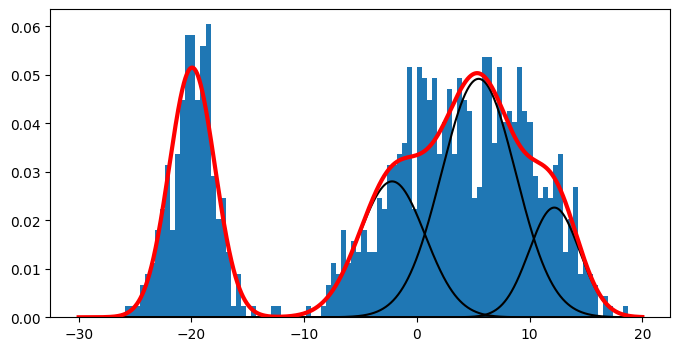
\includegraphics[width=0.9\linewidth]{images/EM1_four_2.png} Ітерація №2: 
%     \par $p=[0.2609, 0.2055, 0.4057, 0.1265],\ $ 
%     $\mu=[-19.9372,  -2.1929,   5.4806,  12.1958],\ $ 
%     $\sigma=[2.0212, 2.9257, 3.2909, 2.2307]$}
% \end{figure}

\begin{figure}[H]
    \center{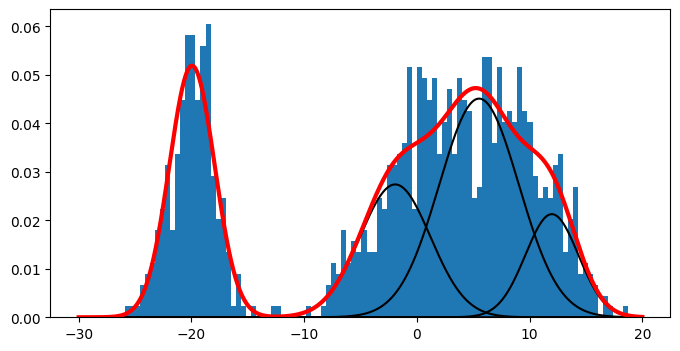
\includegraphics[width=0.9\linewidth]{images/EM1_four_4.png} Ітерація №4: 
    \par $p=[0.2607, 0.2145, 0.3992, 0.1249],\ $ 
    $\mu=[-19.9428,  -1.9204,   5.5187,  11.9785],\ $ 
    $\sigma=[2.0044, 3.1232, 3.5316, 2.3427]$}
\end{figure}

% \begin{figure}[H]
%     \center{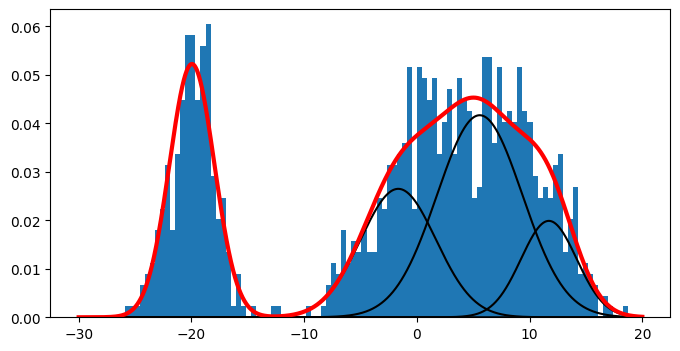
\includegraphics[width=0.9\linewidth]{images/EM1_four_8.png} Ітерація №8: 
%     \par $p=[0.2604, 0.2214, 0.3951, 0.1228],\ $ 
%     $\mu=[-19.9507,  -1.6485,   5.5776,  11.7105],\ $ 
%     $\sigma=[1.9889, 3.3346, 3.7822, 2.4628]$}
% \end{figure}

\begin{figure}[H]
    \center{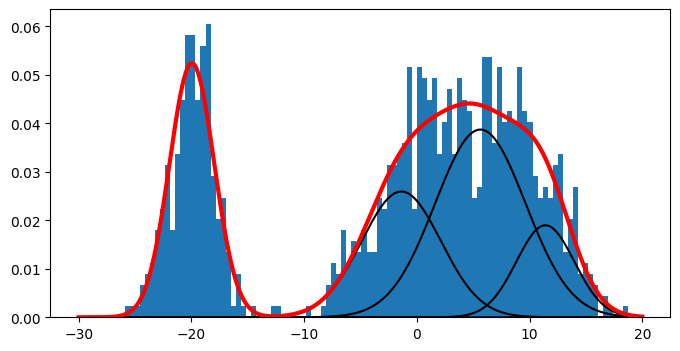
\includegraphics[width=0.9\linewidth]{images/EM1_four_16.png} Ітерація №16: 
    \par $p=[0.2603, 0.2281, 0.3894, 0.1221],\ $ 
    $\mu=[-19.954,   -1.3782,   5.6342,  11.4019],\ $ 
    $\sigma=[1.9826, 3.5079, 4.0118, 2.5686]$}
\end{figure}

% \begin{figure}[H]
%     \center{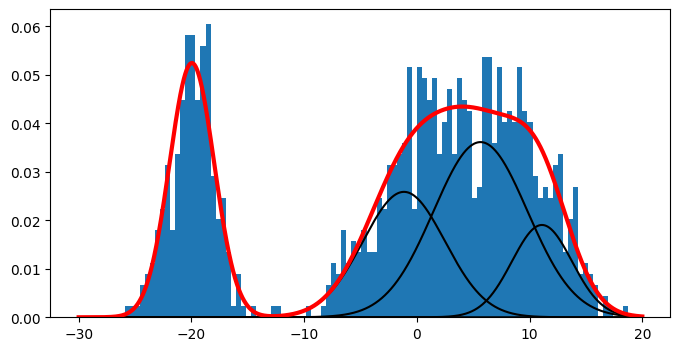
\includegraphics[width=0.9\linewidth]{images/EM1_four_32.png} Ітерація №32: 
%     \par $p=[0.2603, 0.2357, 0.3771, 0.127 ],\ $ 
%     $\mu=[-19.9554,  -1.142,    5.6471,  11.1002],\ $ 
%     $\sigma=[1.98,   3.6342, 4.1635, 2.6606]$}
% \end{figure}

\begin{figure}[H]
    \center{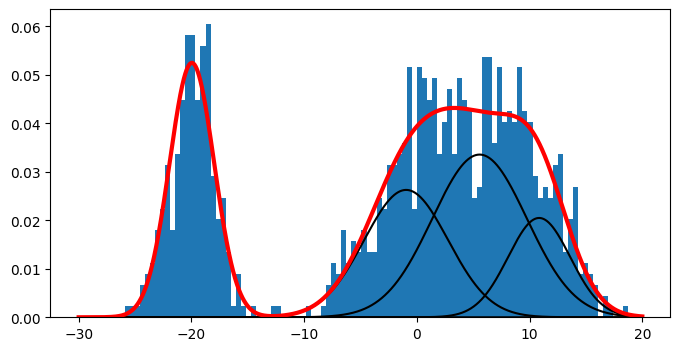
\includegraphics[width=0.9\linewidth]{images/EM1_four_64.png} Ітерація №64: 
    \par $p=[0.2602, 0.245,  0.3533, 0.1415],\ $ 
    $\mu=[-19.9562,  -0.9495,   5.5667,  10.8491],\ $ 
    $\sigma=[1.9787, 3.7211, 4.1995, 2.7564]$}
\end{figure}

Наступними візьмемо, наприклад, такі початкові величини: 
\begin{align*}
    \theta^{(0)} &= \left((p_1^{(0)},p_2^{(0)},p_3^{(0)},p_4^{(0)}), (\mu_1^{(0)},\mu_2^{(0)},\mu_3^{(0)},\mu_4^{(0)}), (\sigma_1^{(0)},\sigma_2^{(0)},\sigma_3^{(0)},\sigma_4^{(0)})\right) \\
    &=\left((0.4,\ 0.2,\ 0.2,\ 0.2),\ (-30, -5,\ 10,\ 10),\ (1,\ 3,\ 3,\ 3)\right)
\end{align*} 

\begin{figure}[H]
    \center{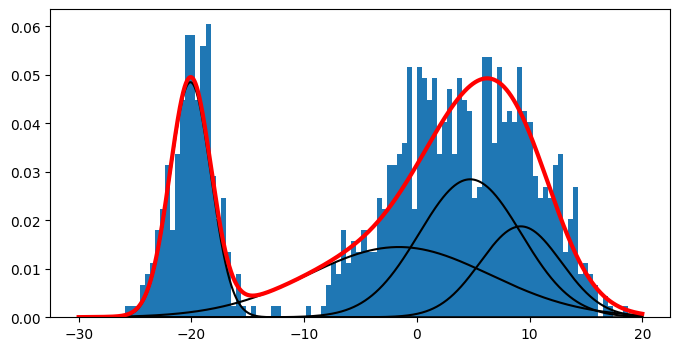
\includegraphics[width=0.9\linewidth]{images/EM2_four_4.png} Ітерація №4: 
    \par $p=[0.2203, 0.2934, 0.3235, 0.169 ],\ $ 
    $\mu=[-20.0842,  -1.5914,   4.7291,   9.2192],\ $ 
    $\sigma=[1.8132, 8.0791, 4.5351, 3.5958]$}
\end{figure}

\begin{figure}[H]
    \center{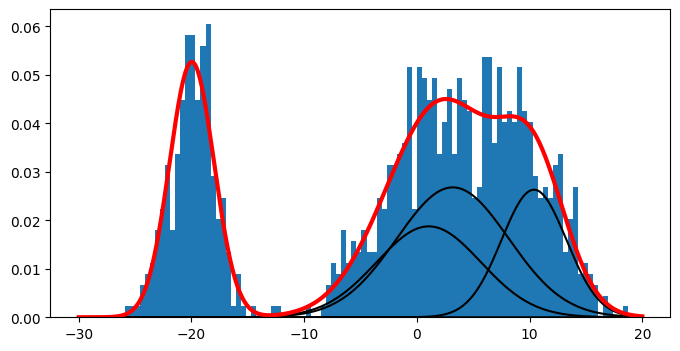
\includegraphics[width=0.9\linewidth]{images/EM2_four_16.png} Ітерація №16: 
    \par $p=[0.26,   0.2174, 0.3333, 0.1898],\ $ 
    $\mu=[-19.962,    1.0557,   3.1866,  10.3907],\ $ 
    $\sigma=[1.9698, 4.6248, 4.9625, 2.8784]$}
\end{figure}

\begin{figure}[H]
    \center{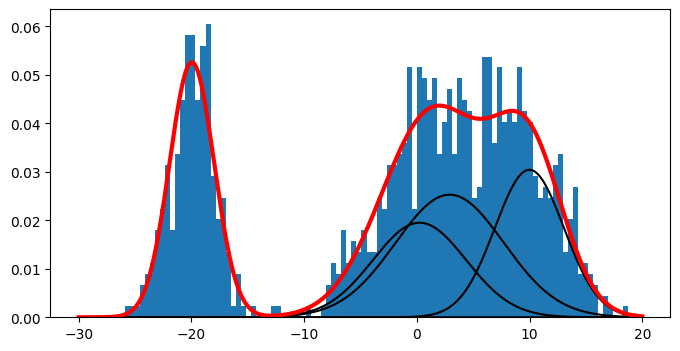
\includegraphics[width=0.9\linewidth]{images/EM2_four_64.png} Ітерація №64: 
    \par $p=[0.2601, 0.2018, 0.3049, 0.2333],\ $ 
    $\mu=[-19.9593,   0.2397,   2.9149,   9.9838],\ $ 
    $\sigma=[1.9736, 4.1279, 4.8099, 3.06  ]$}
\end{figure}

\newpage
І наостанок покладемо $\theta^{(0)}$ таким чином: 
\begin{align*}
    \theta^{(0)} &= \left((p_1^{(0)},p_2^{(0)},p_3^{(0)},p_4^{(0)}), (\mu_1^{(0)},\mu_2^{(0)},\mu_3^{(0)},\mu_4^{(0)}), (\sigma_1^{(0)},\sigma_2^{(0)},\sigma_3^{(0)},\sigma_4^{(0)})\right) \\
    &=\left((0.1,\ 0.5,\ 0.1,\ 0.3),\ (-20,\ 5,\ 5,\ 5),\ (1,\ 4,\ 8,\ 4)\right)
\end{align*} 

\begin{figure}[H]
    \center{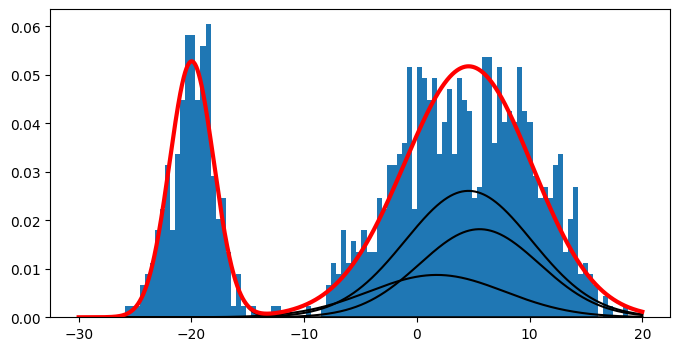
\includegraphics[width=0.9\linewidth]{images/EM3_four_4.png} Ітерація №4: 
    \par $p=[0.2593, 0.3669, 0.1321, 0.2419],\ $ 
    $\mu=[-19.9715,   4.5798,   1.7643,   5.5634],\ $ 
    $\sigma=[1.9602, 5.6141, 6.0358, 5.3111]$}
\end{figure}

\begin{figure}[H]
    \center{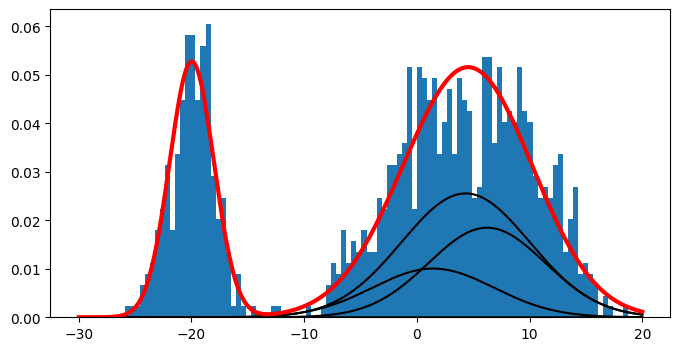
\includegraphics[width=0.9\linewidth]{images/EM3_four_16.png} Ітерація №16: 
    \par $p=[0.2597, 0.3642, 0.136,  0.2401],\ $ 
    $\mu=[-19.9667,   4.3286,   1.4494,   6.2221],\ $ 
    $\sigma=[1.9643, 5.6876, 5.4001, 5.1847]$}
\end{figure}

\begin{figure}[H]
    \center{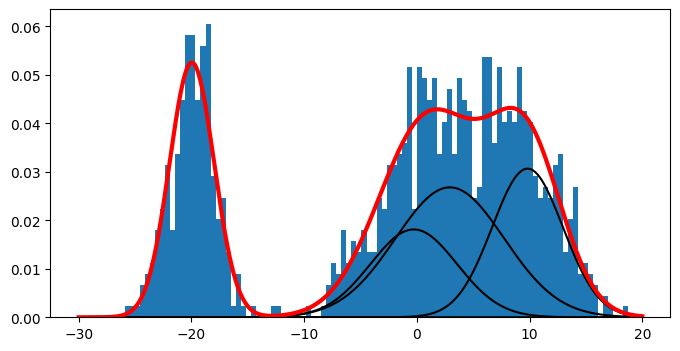
\includegraphics[width=0.9\linewidth]{images/EM3_four_64.png} Ітерація №64: 
    \par $p=[0.2601, 0.3242, 0.1745, 0.2411],\ $ 
    $\mu=[-19.9584,   2.9267,  -0.2773,   9.8184],\ $ 
    $\sigma=[1.9752, 4.8275, 3.8428, 3.1372]$}
\end{figure}

\end{document}